\documentclass{article}
\usepackage{pgfplots}
\usepackage{tikz}
\usepackage{float}
\usepackage{graphicx}
\usepackage{caption}
\usepackage{subcaption}

\usepackage{showframe}
\usepackage[a4paper, margin=3cm]{geometry}
\usetikzlibrary{arrows,decorations.markings}
\usetikzlibrary{shapes, arrows, positioning}
\usetikzlibrary{patterns}
\usetikzlibrary{decorations.pathmorphing,patterns}
\usetikzlibrary{math}
\pgfplotsset{width=15cm, compat=1.15}

\newsavebox{\imagebox}      %za poravnavanje slika i opisa u subfigure 
%\usetikzlibrary{external}
%\tikzexternalize[prefix=meta/]
%\tikzset{external/system call={pdflatex \tikzexternalcheckshellescape -halt-on-error -interaction=batchmode}}

%strelice
\tikzset{strelica1/.style={decoration={markings,mark=at position 1 with %
    {\arrow[scale=2,>=latex']{>}}},postaction={decorate}}}

\tikzset{strelica0/.style={decoration={markings,mark=at position 0 with %
    {\arrow[scale=2,>=latex']{<}}},postaction={decorate}}}

%argumenti #1 - x_0 #2 - y_0 \dx - x_1 #4 - y_1
\newcommand{\prigusivac}[4]{%
    \tikzmath{\dx = #3 - #1;}
    \tikzmath{\dy = #4 - #2;}
    \draw[thick](#1, #2) -- ({\dx/2-0.5}, {\dy/2+#2});
    \draw[thick]({\dx/2-0.5}, {(\dy/2+#2}) -- ({\dx/2-0.1}, {\dy/2+#2});
    \draw[thick]({\dx/2+0.1}, {\dy/2+#2}) -- ({\dx/2+0.5}, {\dy/2+#2});
    \draw[thick]({\dx/2+0.5}, {\dy/2+#2}) -- (#3, #4);

    \draw[thick]({\dx/2-0.1}, {\dy/2+#2-0.3}) -- ({\dx/2-0.1}, {\dy/2+#2+0.3});
    \draw[thick]({\dx/2-0.1}, {\dy/2+#2-0.3}) -- ({\dx/2+0.25}, {\dy/2+#2-0.3});
    \draw[thick]({\dx/2-0.1}, {\dy/2+#2+0.3}) -- ({\dx/2+0.25}, {\dy/2+#2+0.3});

    \draw[thick]({\dx/2+0.1}, {\dy/2+#2+0.2}) -- ({\dx/2+0.1}, {\dy/2+#2-0.2});
}
\begin{document}
\savebox{\imagebox}{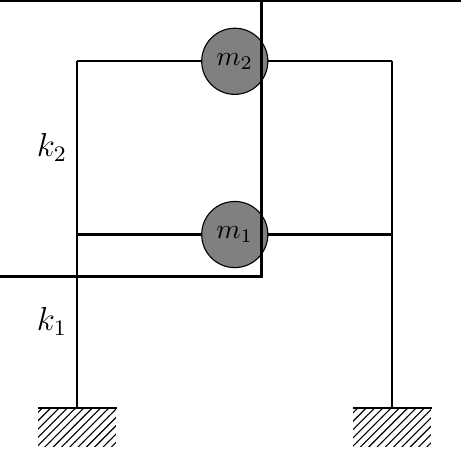
\begin{tikzpicture}
%štapovi
    %prvi (donji) okvir
	\draw[thick] (0,0) -- (0,2.2)
                node[pos=0.5,left]{\large{$k_1$}};
	\draw[thick] (0,2.2) -- (4,2.2);
	\draw[thick] (4,0) -- (4,2.2);

    %drugi (gornji) okvir
        \draw[thick] (0,2.2) -- (0, 4.4)
                node[pos=0.5,left]{\large{$k_2$}};
        \draw[thick] (0, 4.4) -- (4, 4.4);
        \draw[thick] (4, 2.2) -- (4, 4.4);
	
%mase
        %donja
	\filldraw[color=black, fill=gray] (2,2.2) circle (0.42);
	\node[draw=none, fill=none] at(2,2.2) {$m_1$};

        %gornja
        \filldraw[color=black, fill=gray] (2,4.4) circle (0.42);
        \node[draw=none, fill=none] at (2,4.4) {$m_2$};

%podloga
	\draw[white, pattern=north east lines, pattern color=black] (-0.5, 0) 
	rectangle (0.5, -0.5);
	\draw[thick] (-0.5, 0) -- (0.5, 0);

	\draw[white, pattern=north east lines, pattern color=black] (3.5, 0)
	rectangle (4.5, -0.5);
	\draw[thick] (3.5, 0) -- (4.5, 0);
\end{tikzpicture}
}
\begin{figure}[H]
    \begin{subfigure}[b]{0.5\textwidth}
        \centering
        \usebox{\imagebox}
        \caption{Posmični okvir s dva stupnja slobode i prigušenjem}
    \end{subfigure}
    \hfill
    \begin{subfigure}[b]{0.5\textwidth}
        \centering
        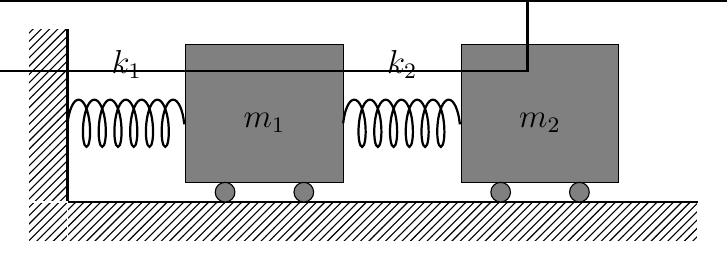
\begin{tikzpicture}
	%podloga
	\draw[white, pattern=north east lines, pattern color=black] (0, 0)
	rectangle (-0.5, 2.2);
	\draw[thick] (0,0) -- (0, 2.2);

	\draw[white, pattern=north east lines, pattern color=black] (0, 0) 
	rectangle (8, -0.5);
	\draw[thick] (0,0) -- (8,0);
	
	\draw[white, pattern=north east lines, pattern color=black] (0, 0)
	rectangle (-0.5, -0.5);

	%uteg
	\filldraw[fill=gray] (1.5, 2) rectangle (3.5, 0.25);
        \filldraw[fill=gray] (5, 2) rectangle (7, 0.25);

	%kotaci
	\filldraw[fill=gray] (2, 0.125) circle (0.125);
	\filldraw[fill=gray] (3, 0.125) circle (0.125);

        \filldraw[fill=gray] (5.5, 0.125) circle (0.125);
        \filldraw[fill=gray] (6.5, 0.125) circle (0.125);

	%opruga
	\draw[thick, decoration={aspect=0.3, segment length=2mm,amplitude=3mm,coil},decorate] (0,1) -- (1.5, 1);
        \draw[thick, decoration={aspect=0.3, segment length=2mm,amplitude=3mm,coil},decorate] (3.5, 1) -- (5, 1);

        \node[draw=none, fill=none] at (0.75, 1.75) {\large{$k_1$}}; 
        \node[draw=none, fill=none] at (2.5,   1) {\large{$m_1$}};

        \node[draw=none, fill=none] at (4.25, 1.75) {\large{$k_2$}};
        \node[draw=none, fill=none] at (6, 1) {\large{$m_2$}};

\end{tikzpicture}

        \caption{Ekvivalentni prigušeni sustav s dva stupnja slobode}
    \end{subfigure}
\end{figure}

\begin{figure}[H]
    \begin{subfigure}[b]{0.5\textwidth}
        \centering
        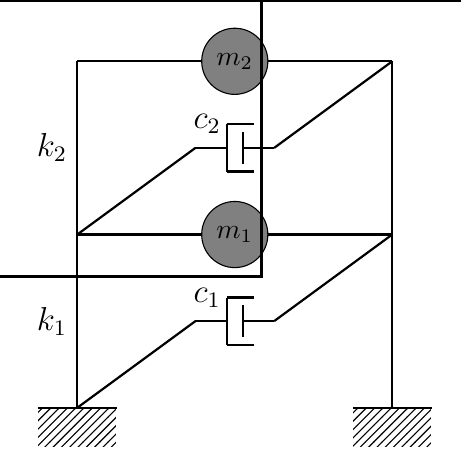
\begin{tikzpicture}
%štapovi
    %prvi (donji) okvir
	\draw[thick] (0,0) -- (0,2.2)
                node[pos=0.5,left]{\large{$k_1$}};
	\draw[thick] (0,2.2) -- (4,2.2);
	\draw[thick] (4,0) -- (4,2.2);

    %drugi (gornji) okvir
        \draw[thick] (0,2.2) -- (0, 4.4)
                node[pos=0.5,left]{\large{$k_2$}};
        \draw[thick] (0, 4.4) -- (4, 4.4);
        \draw[thick] (4, 2.2) -- (4, 4.4);
	
%mase
        %donja
	\filldraw[color=black, fill=gray] (2,2.2) circle (0.42);
	\node[draw=none, fill=none] at(2,2.2) 
        {$m_1$};

        %gornja
        \filldraw[color=black, fill=gray] (2,4.4) circle (0.42);
        \node[draw=none, fill=none] at (2,4.4)
        {$m_2$};

        %dolje
        \prigusivac{0}{0}{4}{2.2}
        \node[draw=none, fill=none] at (1.65, 1.4) {\large{$c_1$}};
        %gore
        \prigusivac{0}{2.2}{4}{4.4} 
        \node[draw=none, fill=none] at (1.65, 3.6) {\large{$c_2$}};


%podloga
	\draw[white, pattern=north east lines, pattern color=black] (-0.5, 0) 
	rectangle (0.5, -0.5);
	\draw[thick] (-0.5, 0) -- (0.5, 0);

	\draw[white, pattern=north east lines, pattern color=black] (3.5, 0)
	rectangle (4.5, -0.5);
	\draw[thick] (3.5, 0) -- (4.5, 0);
\end{tikzpicture}

    \end{subfigure}
    \begin{subfigure}[b]{0.5\textwidth}
        \centering
        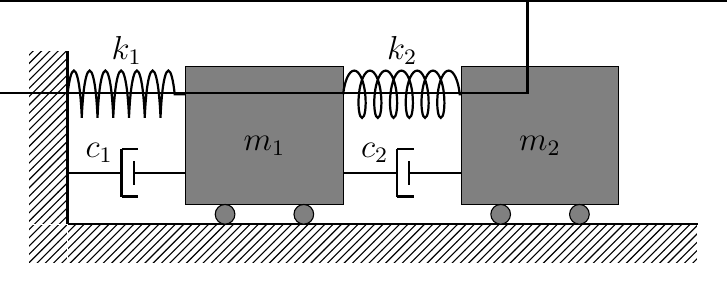
\begin{tikzpicture}
	%podloga
	\draw[white, pattern=north east lines, pattern color=black] (0, 0)
	rectangle (-0.5, 2.2);
	\draw[thick] (0,0) -- (0, 2.2);

	\draw[white, pattern=north east lines, pattern color=black] (0, 0) 
	rectangle (8, -0.5);
	\draw[thick] (0,0) -- (8,0);
	
	\draw[white, pattern=north east lines, pattern color=black] (0, 0)
	rectangle (-0.5, -0.5);

	%uteg
	\filldraw[fill=gray] (1.5, 2) rectangle (3.5, 0.25);
        \filldraw[fill=gray] (5, 2) rectangle (7, 0.25);

	%kotaci
	\filldraw[fill=gray] (2, 0.125) circle (0.125);
	\filldraw[fill=gray] (3, 0.125) circle (0.125);

        \filldraw[fill=gray] (5.5, 0.125) circle (0.125);
        \filldraw[fill=gray] (6.5, 0.125) circle (0.125);

	%opruga
	\draw[thick, decoration={aspect=0.1, segment length=2mm,amplitude=3mm,coil},decorate] (0,1.65) -- (1.5, 1.65);
        \draw[thick, decoration={aspect=0.3, segment length=2mm,amplitude=3mm,coil},decorate] (3.5, 1.65) -- (5, 1.65);

        %prigusivac 1
	\draw[thick] (0, 0.65) -- (0.685, 0.65);
	\draw[thick] (0.84, 0.65) -- (1.5, 0.65);

	\draw[thick] (0.685, 0.35) -- (0.685, 0.95);
	\draw[thick] (0.685, 0.95) -- (0.9, 0.95);
	\draw[thick] (0.685, 0.35) -- (0.9, 0.35);

	\draw[thick] (0.84, 0.5) -- (0.84, 0.8);

        %prigusivac 2 
	\draw[thick] (3.5, 0.65) -- (4.185, 0.65);
	\draw[thick] (4.34, 0.65) -- (5, 0.65);

	\draw[thick] (4.185, 0.35) -- (4.185, 0.95);
	\draw[thick] (4.185, 0.95) -- (4.4, 0.95);
	\draw[thick] (4.185, 0.35) -- (4.4, 0.35);

	\draw[thick] (4.34, 0.5) -- (4.34, 0.8);

        \node[draw=none, fill=none] at (0.75, 2.2) {\large{$k_1$}}; 
        \node[draw=none, fill=none] at (2.5,   1) {\large{$m_1$}};
        \node[draw=none, fill=none] at (0.4,  0.9) {\large{$c_1$}};

        \node[draw=none, fill=none] at (4.25, 2.2) {\large{$k_2$}};
        \node[draw=none, fill=none] at (6, 1) {\large{$m_2$}};
        \node[draw=none, fill=none] at (3.9, 0.9) {\large{$c_2$}};

\end{tikzpicture}

    \end{subfigure}
\end{figure}

\begin{figure}[H]
    \begin{subfigure}[b]{0.5\textwidth}
        \centering
        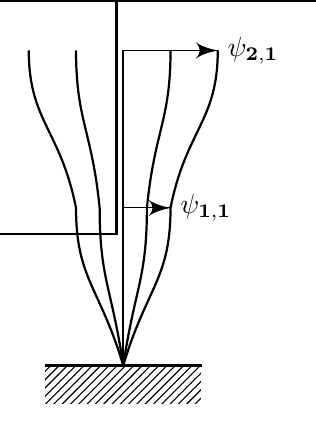
\begin{tikzpicture}
    %podloga
    \draw[white, pattern=north east lines, pattern color=black] (-1, 0)
        rectangle (1, -0.5);
    \draw[thick] (-1, 0) -- (1, 0);

    %centar
    \draw[thick] (0, 0) -- (0, 4);

    %prva
    \draw[thick] (0,0) ..controls (0.3, 1) and (0.6, 1.1).. (0.6, 2);
    \draw[thick] (0.6, 2) ..controls (0.8, 3) and (1.2, 3.1).. (1.2, 4);

    %simetricno
    \draw[thick] (0,0) ..controls (-0.3, 1) and (-0.6, 1.1).. (-0.6, 2);
    \draw[thick] (-0.6, 2) ..controls (-0.8, 3) and (-1.2, 3.1).. (-1.2, 4);

    %druga
    \draw[thick] (0,0) ..controls(0.15, 1) and (0.3, 1.1) .. (0.3, 2);
    \draw[thick] (0.3, 2) ..controls (0.4, 3) and (0.6, 3.1) .. (0.6, 4);

    %simetricno
    \draw[thick] (0,0) ..controls(-0.15, 1) and (-0.3, 1.1) .. (-0.3, 2);
    \draw[thick] (-0.3, 2) ..controls (-0.4, 3) and (-0.6, 3.1) .. (-0.6, 4);

    %vektori
    \draw[strelica1] (0, 2) -- (0.6, 2) node[pos=1,right] {$\mathbf{\psi_{1,1}}$};
    \draw[strelica1] (0, 4) -- (1.2, 4) node[pos=1,right] {$\mathbf{\psi_{2,1}}$};

\end{tikzpicture}

        \caption{Prvi vlastiti oblik titranja sustava s dva stupnja slobode}
    \end{subfigure}
    \hfill
    \begin{subfigure}[b]{0.5\textwidth}
        \centering
        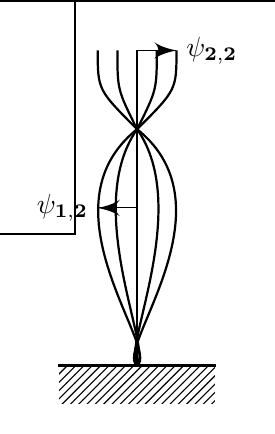
\begin{tikzpicture}
    %podloga
    \draw[white, pattern=north east lines, pattern color=black] (-1, 0)
        rectangle (1, -0.5);
    \draw[thick] (-1, 0) -- (1, 0);

    %centar
    \draw[thick] (0, 0) -- (0, 4);

    %bezier #1
%    \draw[thick] (0,0) ..controls(1.5, 2) and (-0.3,3).. (-0.5, 4);
%    \draw[thick] (0,0) ..controls(-1.5, 2) and (0.3,3).. (0.5, 4);

    \draw[thick] (0, 0) ..controls (0.3, 0.2) and (-1.25, 2) .. (0, 3);
    \draw[thick] (0, 3) ..controls (0.5, 3.5) .. (0.5, 4);

    %simietricno
    \draw[thick] (0, 0) ..controls (-0.3, 0.2) and (1.25, 2) .. (0, 3);
    \draw[thick] (0, 3) ..controls (-0.5, 3.5) .. (-0.5, 4);


    %dvica
    \draw[thick] (0, 0) ..controls (0.2, 0.2) and (-0.7, 2) .. (0, 3);
    \draw[thick] (0, 3) ..controls (0.25, 3.5) .. (0.25, 4);

    %simetricno
    \draw[thick] (0, 0) ..controls (-0.2, 0.2) and (0.7, 2) .. (0, 3);
    \draw[thick] (0, 3) ..controls (-0.25, 3.5) .. (-0.25, 4);

    %vektori
    \draw[strelica1] (0, 2) -- (-0.5, 2) node[pos=1, left] {$\mathbf{\psi_{1,2}}$};
    \draw[strelica1] (0, 4) -- (0.5, 4) node[pos=1, right] {$\mathbf{\psi_{2,2}}$};
\end{tikzpicture}

    \end{subfigure}
\end{figure}

\begin{figure}[H]
    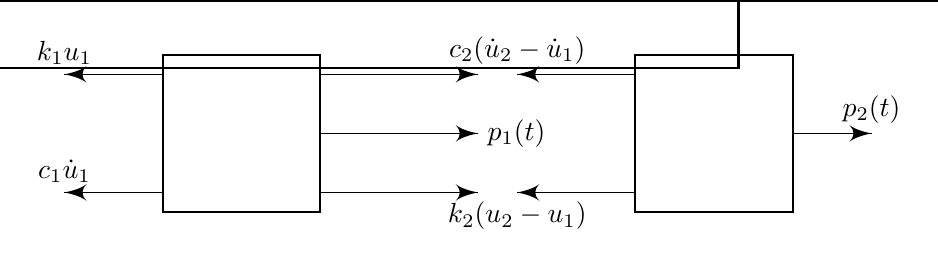
\begin{tikzpicture}
	%uteg_1
	\draw[black,thick] (1.5, 2) rectangle (3.5, 0);

	%sile
	\draw[strelica1] (1.5, 1.75) -- (0.25, 1.75) 
		node[pos=1, above]{$k_1u_1$};
        \draw[strelica1] (1.5, 0.25) -- (0.25, 0.25)
                node[pos=1, above]{$c_1\dot{u}_1$};

	\draw[strelica1] (3.5, 1) -- ( 5.5, 1) 
		node[pos=1, right]{$p_1(t)$};
        \draw[strelica1] (3.5, 1.75) -- (5.5, 1.75);
%                node[pos=1, below]{$k_2(u_2-u_1)$};
        \draw[strelica1] (3.5, 0.25) -- (5.5, 0.25);
%                 node[pos=1, below]{$c_2(\dot{u}_2-\dot{u}_1)$}
                 
            
        %uteg_2
        \draw[black,thick] (7.5, 2) rectangle (9.5, 0);

        %sile
        \draw[strelica1] (7.5, 1.75) -- (6, 1.75)
                node[pos=1, above] {$c_2(\dot{u}_2-\dot{u}_1)$};
        \draw[strelica1] (7.5, 0.25) -- (6, 0.25)
                node[pos=1, below]{$k_2(u_2-u_1)$};
        \draw[strelica1] (9.5, 1) -- (10.5, 1)
                node[pos=1, above]{$p_2(t)$};

\end{tikzpicture}

\end{figure}
\end{document}
